% --------------------------
% ---- DECLARE PACKAGES ----
% --------------------------
\documentclass[a4paper, oneside, openright]{book}
\usepackage[T1]{fontenc} % Font encoding, T1 = it
\usepackage{lmodern}
\usepackage[utf8]{inputenc} % Input encoding - per caratteri particolari
\usepackage[english]{babel} % Lingua principale inglese
\usepackage{blindtext} % Per la generazione di paragrafi lorem ipsum
\usepackage{graphicx} % Per includere immagini esterne
\usepackage[a4paper,top=2.5cm,bottom=2.5cm,left=2.5cm,right=2.5cm]{geometry} %impaginazione e margini documento
\usepackage[fontsize=12pt]{scrextend} %dimensione font
\usepackage[hang,flushmargin]{footmisc} % Disabilita l'indentazione nelle footnotes
\usepackage{titlesec}
\usepackage[newfloat]{minted} % Per i blocchi di codice
\usepackage{float}
\usepackage[font=scriptsize, skip=5pt]{caption} % Spazio tra la caption e l'immagine
\usepackage[backend=biber, style=numeric, defernumbers=true, sorting=none]{biblatex}
\usepackage[immediate]{silence}
\WarningFilter[temp]{latex}{Command} % silence the warning
\usepackage{sectsty}
\DeactivateWarningFilters[temp] % So nothing unrelated gets silenced
\usepackage{hyperref} % Rende l'indice cliccabile
\usepackage[justification=centering]{caption} %per centrare le captions
\usepackage[table,xcdraw]{xcolor}
\usepackage{courier} % font per minted
\usepackage{csquotes} % Dipendenza di babel
\usepackage{acronym}
\usepackage{setspace}
\usepackage{listings}
\usepackage{adjustbox}

% ------------------------
% ---- DOCUMENT SETUP ----
% ------------------------
\pagestyle{plain}
\raggedbottom % Se la pagina non è completa, lascia lo spazio alla fine

\newcommand{\chapnumfont}{%     % define font for chapter number
  \usefont{T1}{pnc}{b}{n}%      % choose New Chancery, bold, normal shape
  \fontsize{85}{100}%          % font size 100pt, baselineskip 100pt
  \vspace{-120pt}               % margin top
  \selectfont%                  % activate font
}

\colorlet{chapnumcol}{gray!75}
\titleformat{\chapter}[display]
{\filleft\bfseries}
{\filleft\chapnumfont\textcolor{chapnumcol}{\thechapter}}
{-24pt}
{\Huge}

\titleformat{name=\chapter, numberless}
{\filleft\bfseries}
{}
{0pt}
{\Huge}[\vspace{45pt}]
\titlespacing*{name=\chapter, numberless}{0pt}{0pt}{0pt}

\hypersetup{ % Setup dell'aspetto dei link
    colorlinks,
    citecolor=black,
    filecolor=black,
    linkcolor=black,
    urlcolor=black
}

\renewcommand{\footnoterule}{ % Rende la linea delle footnotes larga tutta la pagina
  \kern -3pt
  \hrule width \textwidth height 1pt
  \kern 2pt
} 
\renewcommand{\footnotesize}{\fontsize{11pt}{13pt}\selectfont} % Imposta la dimensione del testo delle footnotes
\setlength{\footnotesep}{0.5cm} % Imposta lo spazio fra e singole footnotes
\setlength{\skip\footins}{1.5cm} % Imposta lo spazio fra il corpo e le footnotes

\DeclareUnicodeCharacter{02BC}{}

\newenvironment{code}{\captionsetup{type=listing}}{}
\SetupFloatingEnvironment{listing}{name=Codice}

\usemintedstyle{bw} % setta lo stile dei blocchi minted
\definecolor{bg}{rgb}{0.95,0.95,0.95}

\makeatletter
\AtBeginEnvironment{minted}{\dontdofcolorbox}
\def\dontdofcolorbox{\renewcommand\fcolorbox[4][]{##4}}
\makeatother

\newcommand*\blankpage{\newpage\null\thispagestyle{empty}\newpage}

% ------------------------
% ---- DOCUMENT START ----
% ------------------------
\addbibresource{bibliography.bib} % Importiamo la bibliografia
\begin{document} % Inizio documento
\pagenumbering{gobble} % Disabilita numerazione pagine
\begin{titlepage}
	\centering
    %\vspace*{0.5 cm}
    \textsc{Università degli Studi di Milano-Bicocca \\ Dipartimento di Informatica, Sistemistica e Comunicazione}\\[2.0 cm]	% University Name
    \vspace*{3 cm}
    %\includegraphics[scale = 0.30]{images/redis_logo.png}\\[1.0 cm]	% University Logo
    \rule{\linewidth}{0.2 mm} \\[1.5 cm]
	{ \huge \bfseries Wi-Fi Hacking: Attacks on WPA2 and Unsecured Communications}\\
    \vspace*{2.0 cm}
    \rule{\linewidth}{0.2 mm} \\[1.5 cm]
    \textsc{Cybersecurity Course A.A.2024/2025}\\[1.5 cm]				% Course Code
    
    \vspace*{4 cm}
	
	\begin{minipage}{0.4\textwidth}
		\begin{flushleft} \large
			\end{flushleft}
			\end{minipage}~
			\begin{minipage}{0.4\textwidth}
            
		\begin{flushright} \large
			\emph{Author:} \\
			Pulcino Federico\\
            Student ID 872491\\
		\end{flushright}
        
	\end{minipage}\\[2 cm]
 
\end{titlepage} % PAGINA FRONTESPIZIO
\newpage % Nuova pagna
\setcounter{chapter}{0} % Fa risultare l'introduzione come capitolo 0
%\input{Dedica}
\tableofcontents

%\chapter*{Lista degli acronimi} % acronym 
%\input{acronyms.tex} 
%\blankpage
\newpage % Nuova pagna
\pagenumbering{arabic} % Riabilita la numerazione in modo che cominci dal primo capitolo
% ------------------
% ---- CHAPTERS ----
% ------------------
\chapter{Introduction}

This project serves as an in-depth exploration of the security challenges and vulnerabilities associated with WPA2 (Wi-Fi Protected Access 2), one of the most widely used protocols for securing wireless networks. WPA2, based on the Advanced Encryption Standard (AES), provides robust mechanisms for ensuring data confidentiality and integrity. However, practical implementations of this protocol are not immune to targeted attacks, making it critical to understand both its strengths and weaknesses.

The study is structured around three interconnected simulations, each highlighting a specific aspect of wireless network security:

\begin{enumerate}
    \item \textbf{Exploring WPA2 Handshake Vulnerabilities}: The first simulation focuses on capturing and analyzing the WPA2 four-way handshake, demonstrating how adversaries can exploit weaknesses in passphrase selection through brute-force attacks using precompiled dictionaries. This experiment underscores the importance of strong, complex passwords in mitigating such risks.

    \item \textbf{Evil Twin Attack Simulation}: The second simulation illustrates the creation of an Evil Twin access point, a common phishing attack designed to deceive users into connecting to a rogue network. By mimicking a legitimate network, the attacker can intercept sensitive data, emphasizing the critical need for user awareness and advanced authentication mechanisms.

    \item \textbf{Data Transmission in Unencrypted Networks}: The final simulation examines the risks of open networks, where data is transmitted in plain text. By hosting a simple HTTP form on an attacker device and capturing traffic using Wireshark, the study reveals how sensitive information, such as usernames and passwords, can be intercepted when encryption is absent.
\end{enumerate}

Through these simulations, conducted in a controlled environment using open-source tools such as Aircrack-ng and Wireshark, this project bridges theoretical concepts with practical applications. The findings provide a comprehensive understanding of wireless network vulnerabilities and underscore the necessity of adopting modern security protocols, such as WPA3, and following best practices to safeguard against emerging threats.

This report integrates technical analyses with hands-on experimentation, offering insights into the complexities of wireless security and the ongoing efforts required to ensure robust protection in real-world scenarios.

\part{Theoretical Knowledge}
\chapter{Overview of WPA2 and the Four-Way Handshake}
Wi-Fi Protected Access II (WPA2) is the second generation of the WPA security protocol, designed to secure wireless networks. Based on the IEEE 802.11i standard, WPA2 became mandatory for all Wi-Fi-certified devices starting in 2006. This protocol addresses significant vulnerabilities found in its predecessor, WPA, and introduces critical security enhancements that ensure robust encryption and data integrity.

\section{Key Features of WPA2}
WPA2 offers several key improvements over WPA, the most notable of which are enhanced encryption, improved data integrity, and mandatory certification. These advancements make WPA2 a trusted solution for both enterprise and personal wireless network security.

\begin{itemize}
    \item \textbf{Enhanced Encryption}: WPA2 replaces WPA's Temporal Key Integrity Protocol (TKIP) with the Counter Mode Cipher Block Chaining Message Authentication Code Protocol (CCMP). CCMP leverages the Advanced Encryption Standard (AES), a much stronger encryption algorithm that uses a 128-bit key. AES ensures higher levels of confidentiality and integrity for transmitted data, providing resistance against brute-force attacks and cryptographic weaknesses.
    
    \item \textbf{Improved Data Integrity}: WPA2 employs CCMP for message integrity, replacing the weaker Message Integrity Code (MIC) used in WPA. CCMP ensures that data cannot be altered or tampered with during transmission, thereby preventing attacks such as packet injection or replay attacks. The shift to AES-based encryption and a more robust integrity mechanism enhances overall network security.
    
    \item \textbf{Mandatory Certification and Testing}: WPA2 certification, enforced by the Wi-Fi Alliance, ensures that devices meet the rigorous security standards required for Wi-Fi networks. Since March 2006, all Wi-Fi-certified devices have been required to support WPA2, making it the default security protocol for most wireless devices.
\end{itemize}

\section{How WPA2 Works: The Four-Way Handshake}
The primary method by which WPA2 ensures secure communication between clients (stations) and access points (APs) is through the Four-Way Handshake. This handshake is essential for establishing a secure communication session by verifying the legitimacy of both parties and generating the necessary encryption keys.

The Four-Way Handshake is designed to prevent eavesdropping, man-in-the-middle attacks, and replay attacks, and to ensure the integrity of the encryption keys used in communication. Below is a detailed explanation of the handshake process:

\subsection{Key Concepts}
To understand the Four-Way Handshake, it is important to first define several key cryptographic elements involved in the process:

\begin{itemize}
    \item \textbf{PMK (Pairwise Master Key)}: The PMK is derived from the pre-shared key (PSK) or, in enterprise networks, from an 802.1X authentication server. It is a 256-bit key that serves as the root key for generating other session keys used in the handshake process.
    
    \item \textbf{PTK (Pairwise Transient Key)}: The PTK is the key used to encrypt unicast traffic between the client and the AP. It is derived from the PMK, as well as random values (nonces) generated by both parties.
    
    \item \textbf{GTK (Group Temporal Key)}: The GTK is used to encrypt multicast and broadcast traffic between the AP and its clients. It is generated by the AP and shared with all clients connected to the network.
    
    \item \textbf{ANONCE and SNONCE}: These are random nonces generated by the AP and client, respectively. They play a critical role in ensuring the freshness of the session and preventing replay attacks.
    
    \item \textbf{MIC (Message Integrity Code)}: The MIC is a cryptographic checksum used to ensure the integrity of the messages exchanged during the handshake. It prevents tampering and assures both parties that the data has not been modified.
\end{itemize}

\subsection{The Four-Way Handshake Process}
The Four-Way Handshake consists of four messages exchanged between the client and the AP, during which the cryptographic keys necessary for securing the connection are derived and exchanged. The process can be broken down as follows:

\begin{enumerate}
    \item \textbf{Message 1 (AP to Client)}: The AP sends a message containing its nonce (ANONCE) to the client. This nonce is required by the client to generate the Pairwise Transient Key (PTK). At this point, the client already has the pre-shared key (PSK), which is used to derive the Pairwise Master Key (PMK).
    
    \item \textbf{Message 2 (Client to AP)}: The client generates its own nonce (SNONCE) and sends it to the AP, along with a Message Integrity Code (MIC). The MIC is a cryptographic signature that allows the AP to verify that the message is legitimate and originated from the client. Upon receiving the message, the AP derives the PTK, using the PMK, ANONCE, SNONCE, and the MAC addresses of both the AP and the client.
    
    \item \textbf{Message 3 (AP to Client)}: The AP sends the Group Temporal Key (GTK) to the client. The GTK is used for encrypting multicast and broadcast traffic, ensuring that all clients on the same AP can securely communicate. The client installs the GTK, which allows it to handle group traffic.
    
    \item \textbf{Message 4 (Client to AP)}: The client sends a confirmation message to the AP, indicating that it has successfully installed both the PTK and GTK. This final step completes the handshake and secures the communication channel between the client and the AP.
\end{enumerate}

The exchange of these four messages establishes a secure session, where the PTK is used for unicast traffic encryption, and the GTK is used for broadcast and multicast traffic encryption.

\section{Security Implications and Cracking WPA2}
The WPA2 Four-Way Handshake plays a crucial role in maintaining the security of wireless networks. However, the handshake's reliance on the pre-shared key (PSK) means that the strength of the security depends heavily on the strength of the password chosen by the network administrator. 

An attacker can exploit the handshake process by capturing the messages exchanged between the client and the AP. One common method is to force a client to disconnect and reconnect, thereby triggering a new handshake. Once captured, the attacker can attempt to crack the pre-shared key (PSK) by performing a brute-force attack using tools like \textbf{aircrack-ng}.





\part{Practical Implementation}
\chapter{Enviroment}
\section{Hardware Specification}
The hardware utilized for the testing environment comprised a laptop with specifications tailored to meet the requirements of wireless network testing, particularly for WPA2 security evaluation. The primary device used was an \textbf{ASUS ZenBook UX331U} with the following hardware configuration:

\begin{itemize}
    \item \textbf{Processor:} Intel\textsuperscript{\textregistered} Core\texttrademark\ i7-8550U Processor, featuring 4 cores and a base clock speed of 1.8 GHz, with a turbo boost up to 4.0 GHz, and an 8 MB cache.
    \item \textbf{Memory:} 8 GB of RAM, ensuring smooth performance for resource-intensive tasks such as packet capture and traffic analysis.
    \item \textbf{Wireless Network Interface:} Intel\textsuperscript{\textregistered} Dual Band Wireless-AC 8265 module, which supports:
    \begin{itemize}
        \item \textbf{TX/RX Streams:} 2x2
        \item \textbf{Frequency Bands:} Dual-band operation at 2.4 GHz and 5 GHz.
        \item \textbf{Maximum Speed:} Up to 867 Mbps, compliant with the Wi-Fi 5 (802.11ac) standard.
    \end{itemize}
\end{itemize}

\section{Operating System}

For this project, I used \textbf{Kali Linux} version 2024.3, running in \textit{Live USB} mode with \textbf{data persistence} enabled. This configuration allowed me to work directly from a USB drive while saving changes and settings between sessions, making it practical for repeated testing without the need to reconfigure the environment every time.

Kali Linux is a specialized operating system designed for penetration testing and cybersecurity tasks. It comes with a wide range of pre-installed tools, such as \textit{airmon-ng}, \textit{aircrack-ng}, and \textit{Wireshark}, which were essential for capturing WPA2 handshakes, analyzing network traffic, and simulating attacks. 

Using a persistent Live USB setup ensured flexibility and portability while maintaining a stable testing environment. This approach was particularly useful for experimenting with different configurations and tools specific to the project without affecting the main operating system on my laptop.



\chapter{Deauthentication Attack and WPA2 Handshake Capture}

This chapter outlines the practical execution of the deauthentication attack with the aim of capturing the WPA2 handshake. This method is commonly used in wireless network penetration testing to demonstrate how WPA2 can be compromised, especially when weak passwords are used.

\section{Introduction to the Deauthentication Attack}
The deauthentication attack targets connected wireless clients by sending deauthentication frames that force them to disconnect from their access point (AP). As soon as the client tries to reconnect, the WPA2 handshake is transmitted, and if captured, it can be used to attempt password recovery through brute-force or dictionary attacks.

This attack exploits the fact that deauthentication frames are not authenticated, meaning they can be easily spoofed by any device within range, making it possible for an attacker to force clients to disconnect from the network. This triggers the WPA2 handshake process, which can then be captured for further analysis.

\subsection{Tools and Software Utilized}
This section provides an overview of the tools and software employed during the practical execution of the deauthentication attack and WPA2 handshake capture. Each tool played a critical role in various stages of the attack, from configuring the network interface to analyzing the captured handshake.

\subsubsection{Airmon-ng}
Part of the `aircrack-ng` suite, `airmon-ng` is a tool used to enable and manage monitor mode on wireless network interfaces. In this experiment, it was employed to switch the wireless adapter into monitor mode, allowing it to capture all wireless traffic within range. Additionally, it was used to terminate interfering processes to ensure a smooth operation during packet capture.

\subsubsection{Airodump-ng}
`Airodump-ng` is another utility within the `aircrack-ng` suite, designed for packet capture and real-time analysis of wireless traffic. It was instrumental in scanning for nearby networks, identifying the target access point, and capturing the WPA2 handshake during the attack.

\subsubsection{Aireplay-ng}
`Aireplay-ng` is a packet injection tool used to perform various wireless network attacks, including deauthentication attacks. In this experiment, it was utilized to send deauthentication frames to force connected clients to disconnect from the target access point, thereby triggering the WPA2 handshake.

\subsubsection{Aircrack-ng}
The `aircrack-ng` tool is the centerpiece of the suite, specializing in wireless network password cracking. In this scenario, it was used to execute the dictionary attack on the captured WPA2 handshake. By iterating through the entries in the `rockyou.txt` wordlist, `aircrack-ng` successfully recovered the network password.

\subsubsection{Wireshark}
Wireshark is a versatile network protocol analyzer used for inspecting captured network traffic in detail. After capturing the WPA2 handshake, Wireshark was employed to verify the integrity of the handshake and confirm that all necessary packets were captured correctly.

\subsubsection{RockYou Dictionary}
The `rockyou.txt` dictionary is a widely known wordlist containing millions of commonly used passwords. It served as the dictionary for the password-cracking phase, highlighting the risks associated with weak and commonly used passwords.

Each of these tools contributed to the successful execution of the attack, from capturing wireless traffic to analyzing and recovering the network password. Their combined functionality underscores the importance of understanding and mitigating these vulnerabilities in wireless network security.


\section{Objective and Methodology for Capturing the WPA2 Handshake}
The primary goal of this section is to capture the WPA2 handshake between a client and the AP using the deauthentication attack. The following steps outline the process and the commands used for execution:

\begin{enumerate}
    \item \textbf{Switching the Network Interface to Monitor Mode:} The first step in preparing for the deauthentication attack is to enable monitor mode on the wireless adapter, which allows the interface to capture all wireless traffic within range. As illustrated in Figure \ref{fig:wlanmon}, I began by checking the current state of the wireless interface using the command \textit{iwconfig}. To ensure that no processes would interfere with the monitor mode, I terminated any conflicting processes using the command \textit{sudo airmon-ng check kill}. Finally, I switched the wireless card into monitor mode with the command \textit{sudo airmon-ng start wlan0}, which reconfigures the adapter from managed to monitor mode, enabling it to capture all nearby wireless packets.

    \begin{figure}[h!]
        \centering
        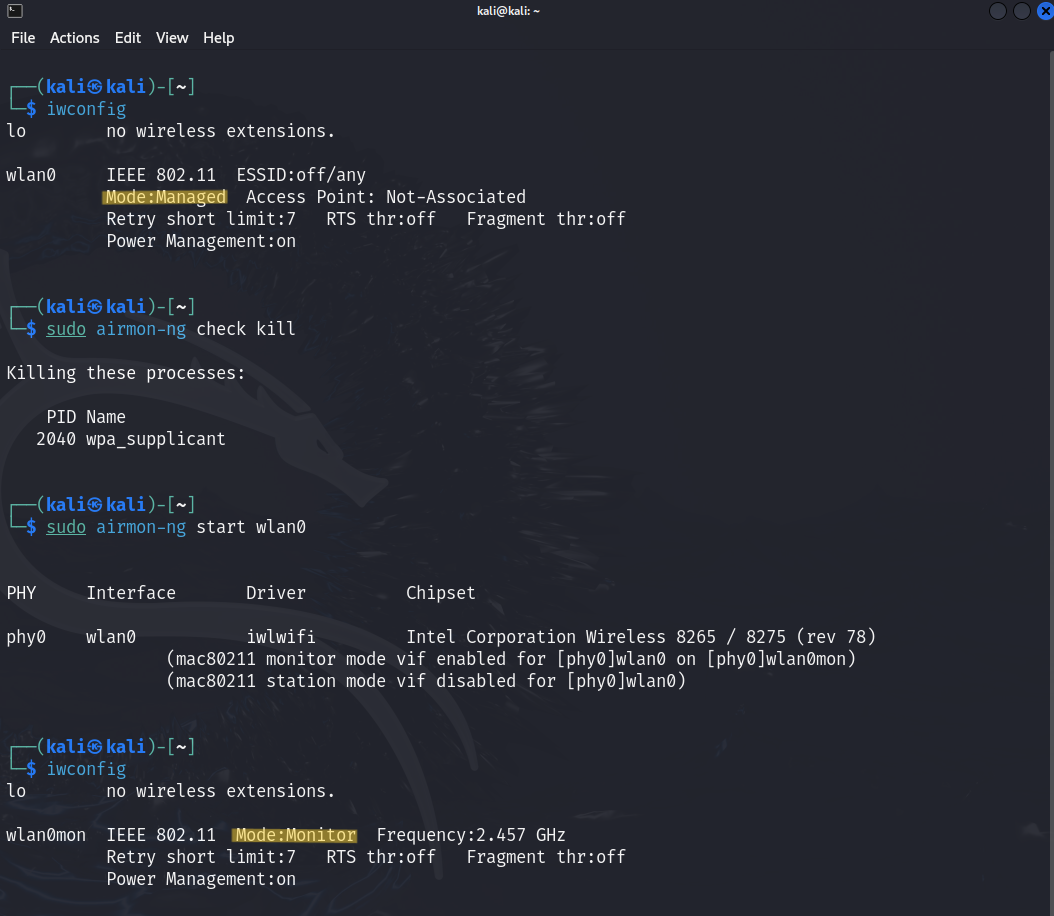
\includegraphics[width=0.8\linewidth]{images/wlanmon.png}
        \caption{Monitor mode enabled on the wireless card.}
        \label{fig:wlanmon}
    \end{figure}

    \item \textbf{Scanning for Nearby Networks:} Once the network interface was in monitor mode, the next step was to scan for nearby wireless networks. This was accomplished using the command \textit{sudo airodump-ng wlan0mon}.

    As shown in Figure \ref{fig:networklist}, this command provides a list of all available access points, displaying details such as the BSSID (MAC address), channel, encryption type, and the number of connected clients. From this list, I was able to identify the target network, along with its corresponding BSSID and channel.

    \begin{figure}[h!]
        \centering
        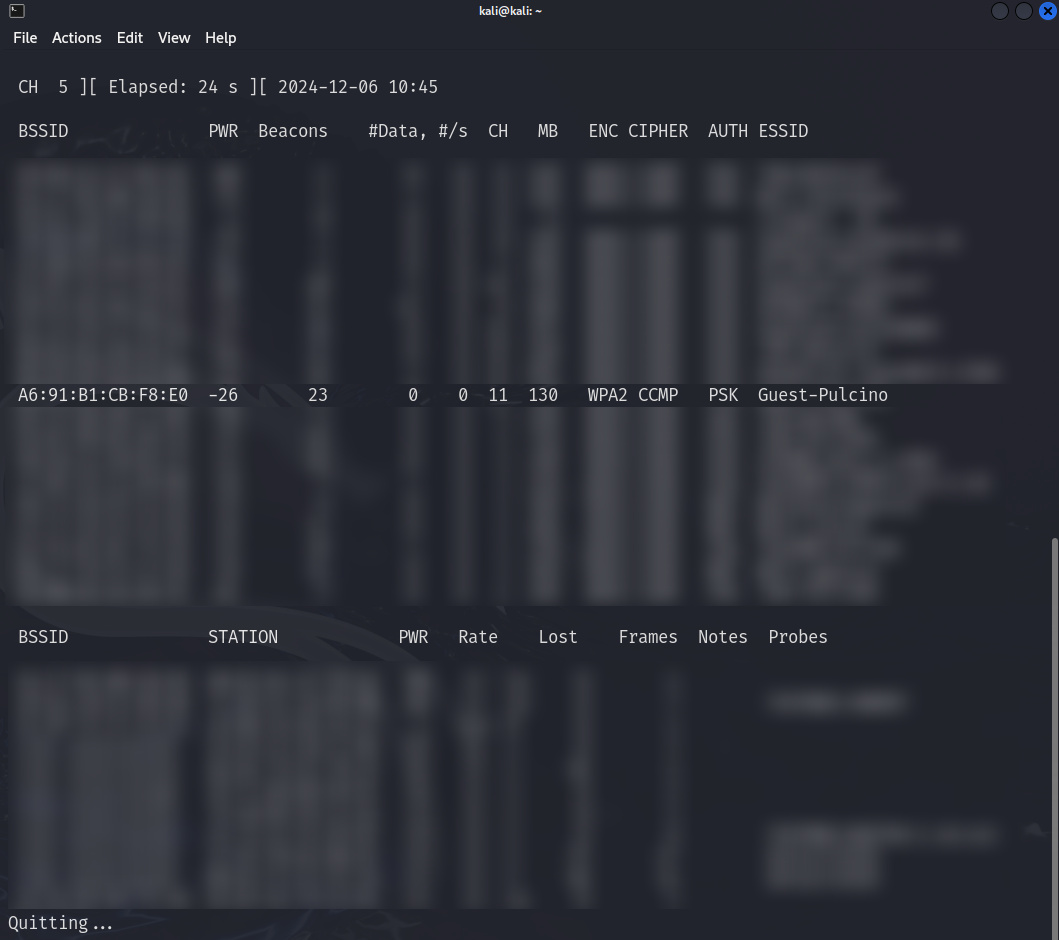
\includegraphics[width=0.8\linewidth]{images/networklist.png}
        \caption{List of nearby networks and stations.}
        \label{fig:networklist}
    \end{figure}

    At this stage, I had successfully identified the BSSID and channel of my target network.

    \item \textbf{Identifying the Target Network:} After identifying the target network, the next step was to focus the attack on the specific channel used by the target access point. To filter the results and capture only the traffic from the target network, I used the following command: \textit{"sudo airodump-ng --bssid A6:91:B1:CB:F8:E0 -c 11 -w wificapture wlan0"}. In this command, the \textit{-w wificapture} flag specifies the filename where the captured handshake will be saved, and the \textit{-c 11} flag ensures that only traffic on channel 11, where the target AP operates, is captured. The results are displayed in Figure \ref{fig:handshakelistening}.

    \begin{figure}[h!]
        \centering
        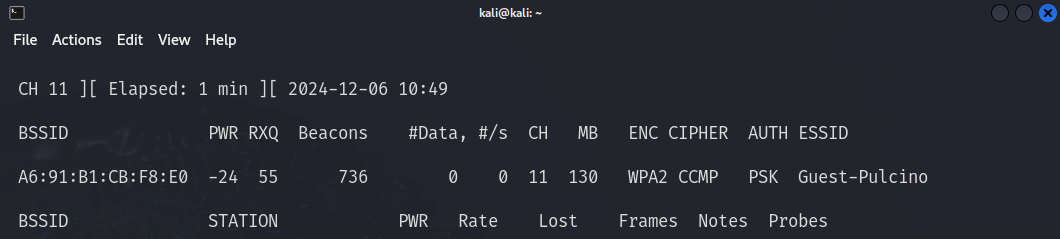
\includegraphics[width=0.8\linewidth]{images/handshakelistening.png}
        \caption{Listening for the handshake on the target network.}
        \label{fig:handshakelistening}
    \end{figure}

    \item \textbf{Sending Deauthentication Frames:} With the target network identified and the capture in progress, the next step was to send deauthentication frames to disconnect any connected clients from the access point. As shown in Figure \ref{fig:deauth}, this was achieved using the following command: \textit{"sudo aireplay-ng --deauth 0 -a A6:91:B1:CB:F8:E7 wlan0mon"}. The \textit{--deauth 0} flag indicates that deauthentication packets will be sent indefinitely (until manually stopped). These frames force the connected devices to disconnect and attempt to reconnect, which triggers the WPA2 handshake.

    \begin{figure}[h!]
        \centering
        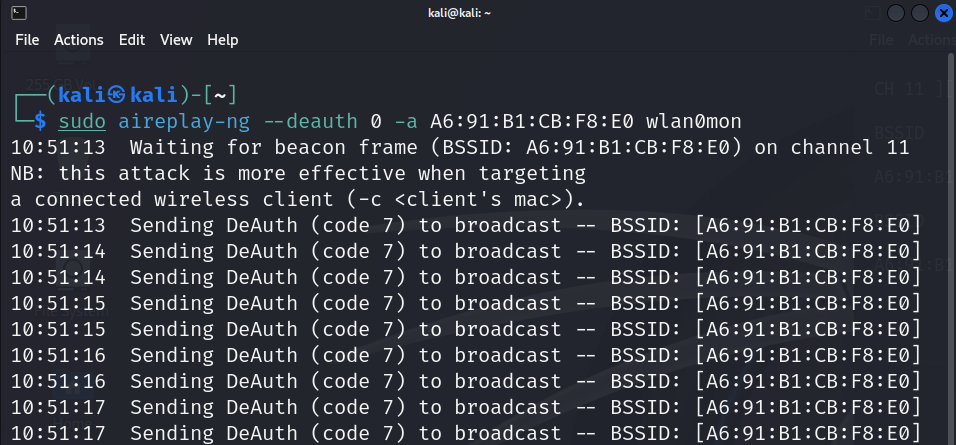
\includegraphics[width=0.8\linewidth]{images/dauth.png}
        \caption{Deauthentication packets being sent.}
        \label{fig:deauth}
    \end{figure}

    \item \textbf{Capturing the WPA2 Handshake:} When a client attempts to reconnect to the access point, the WPA2 handshake is triggered and captured by the \textit{airodump-ng} tool. This handshake is crucial for subsequent analysis. Once the handshake capture is complete, the tool provides confirmation in the form of output, as shown in Figure \ref{fig:handshakecaputred}.

    \begin{figure}[h!]
        \centering
        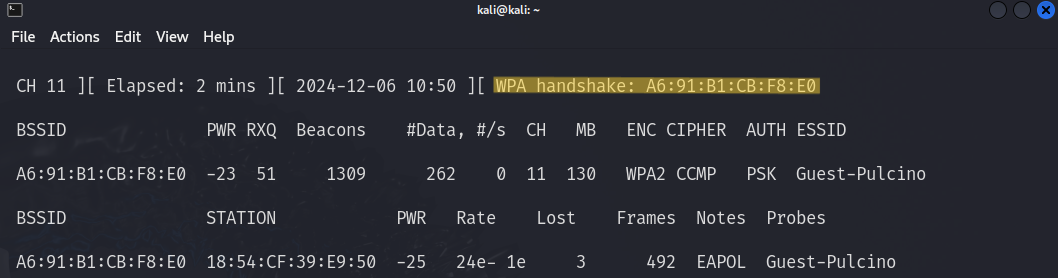
\includegraphics[width=0.8\linewidth]{images/handshakecaptured.png}
        \caption{WPA2 handshake successfully captured.}
        \label{fig:handshakecaputred}
    \end{figure}
    
    The captured handshake is then saved to the specified file, ready for further analysis or potential use in an attack.

    \item \textbf{Analyzing the Handshake:} The captured handshake was analyzed using \texttt{Wireshark} to verify its completeness and to understand the cryptographic exchanges between the client and the AP. As outlined in the theoretical section, the WPA2 handshake consists of four messages that establish the Pairwise Transient Key (PTK) and the Group Temporal Key (GTK), ensuring secure communication between the two parties.

\begin{enumerate}
    \item \textbf{Message 1:} The AP sends a random nonce (\texttt{ANONCE}) to the client. This nonce, shown in Figure \ref{fig:msg1}, is crucial for the client to derive the PTK using the pre-shared key (PSK) and other parameters.
    \begin{figure}[h!]
        \centering
        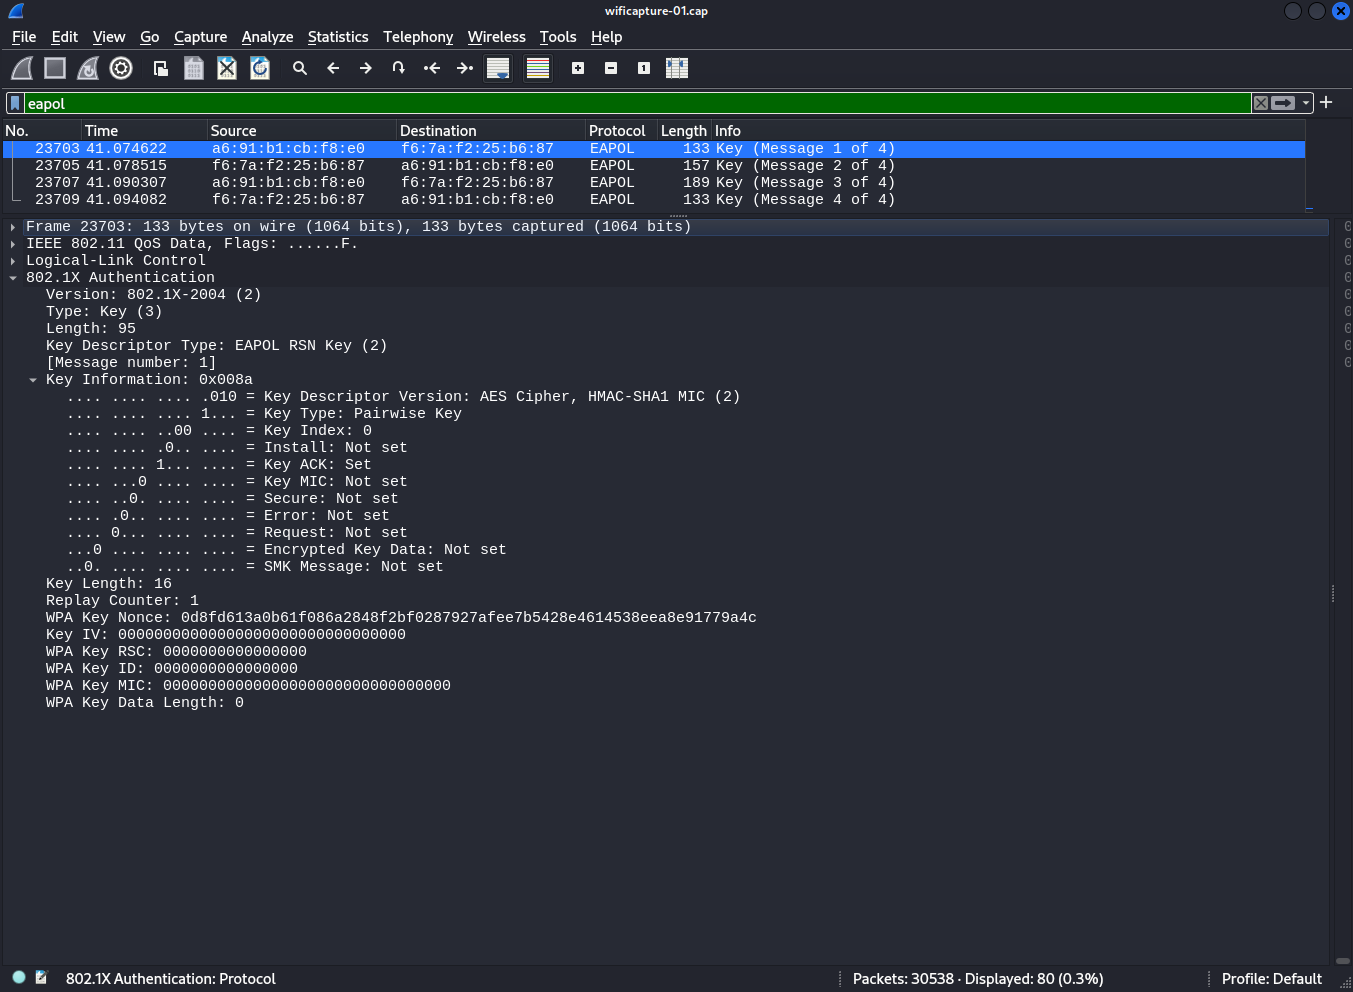
\includegraphics[width=0.8\linewidth]{images/msg1.png}
        \caption{Message 1: AP sending ANONCE to the client.}
        \label{fig:msg1}
    \end{figure}

    \item \textbf{Message 2:} The client responds with its own nonce (\texttt{SNONCE}) and a Message Integrity Code (MIC) to ensure the integrity of the exchange. As depicted in Figure \ref{fig:msg2}, this step confirms the client’s identity and provides the AP with the data needed to compute the PTK.
    \begin{figure}[h!]
        \centering
        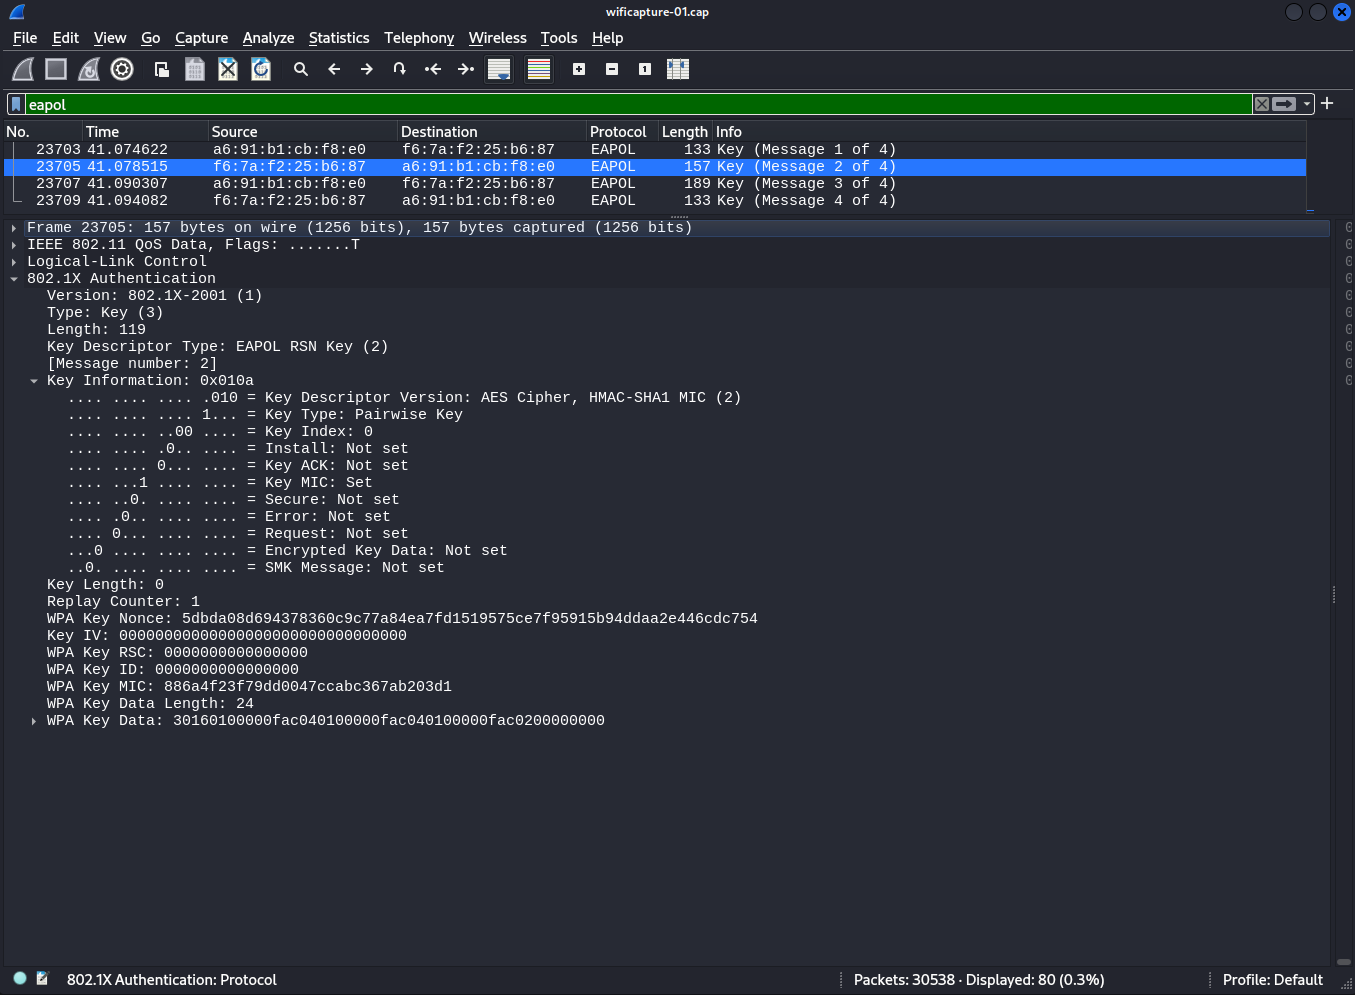
\includegraphics[width=0.8\linewidth]{images/msg2.png}
        \caption{Message 2: Client sending SNONCE and MIC to the AP.}
        \label{fig:msg2}
    \end{figure}

    \item \textbf{Message 3:} The AP transmits the Group Temporal Key (GTK) to the client, ensuring that all clients on the network can securely communicate in multicast and broadcast traffic. This can be seen in Figure \ref{fig:msg3}.
    \begin{figure}[h!]
        \centering
        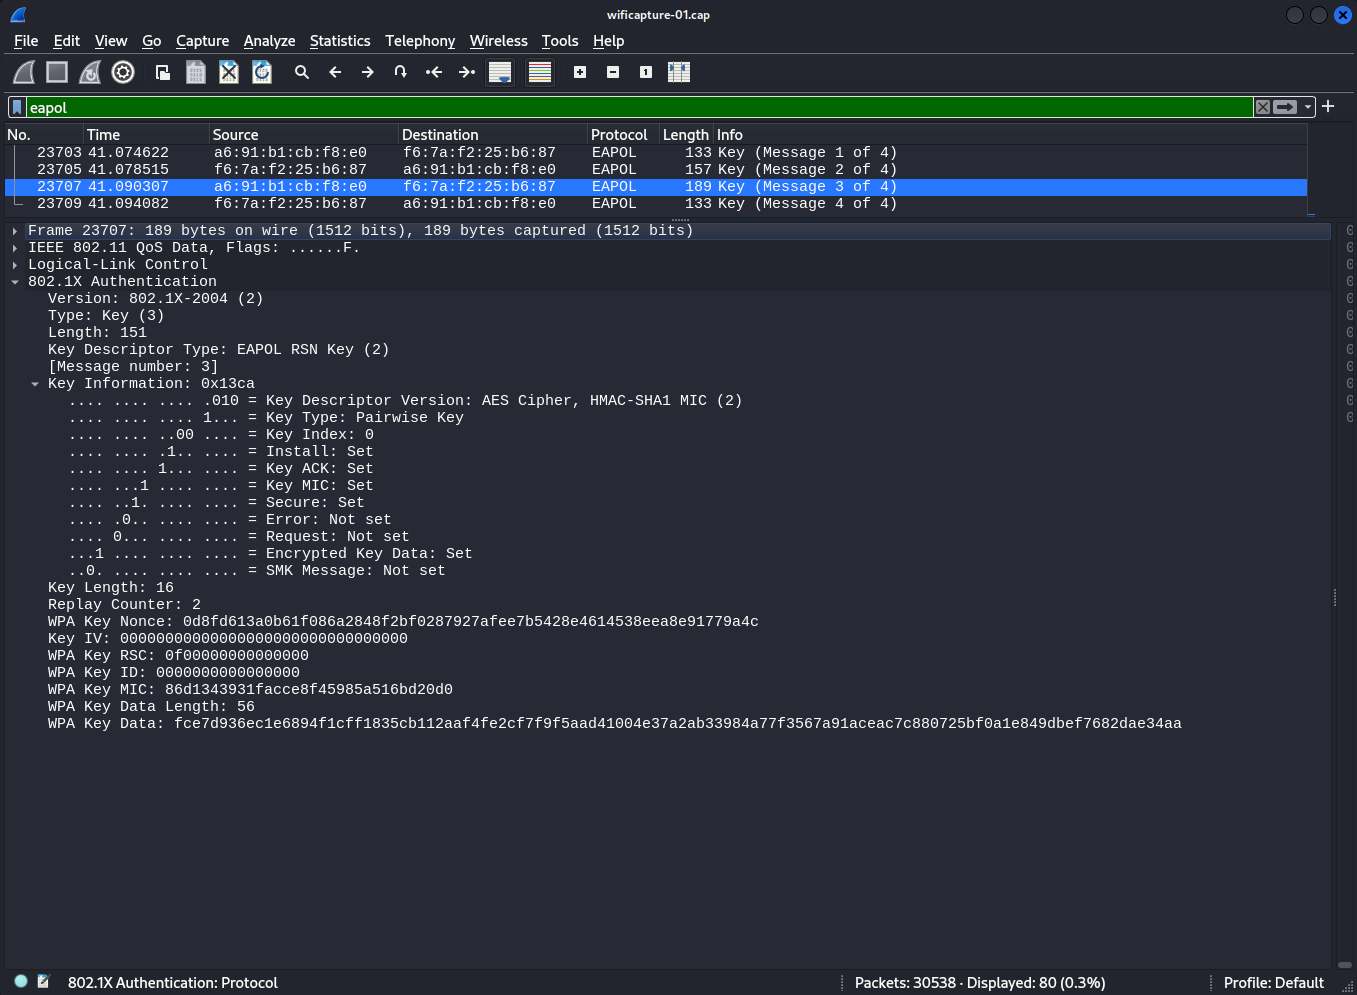
\includegraphics[width=0.8\linewidth]{images/msg3.png}
        \caption{Message 3: AP sending GTK to the client.}
        \label{fig:msg3}
    \end{figure}

    \item \textbf{Message 4:} The client sends a final acknowledgment to the AP, confirming the installation of the PTK and GTK. This step, illustrated in Figure \ref{fig:msg4}, completes the handshake process, establishing a secure communication channel.
    \begin{figure}[h!]
        \centering
        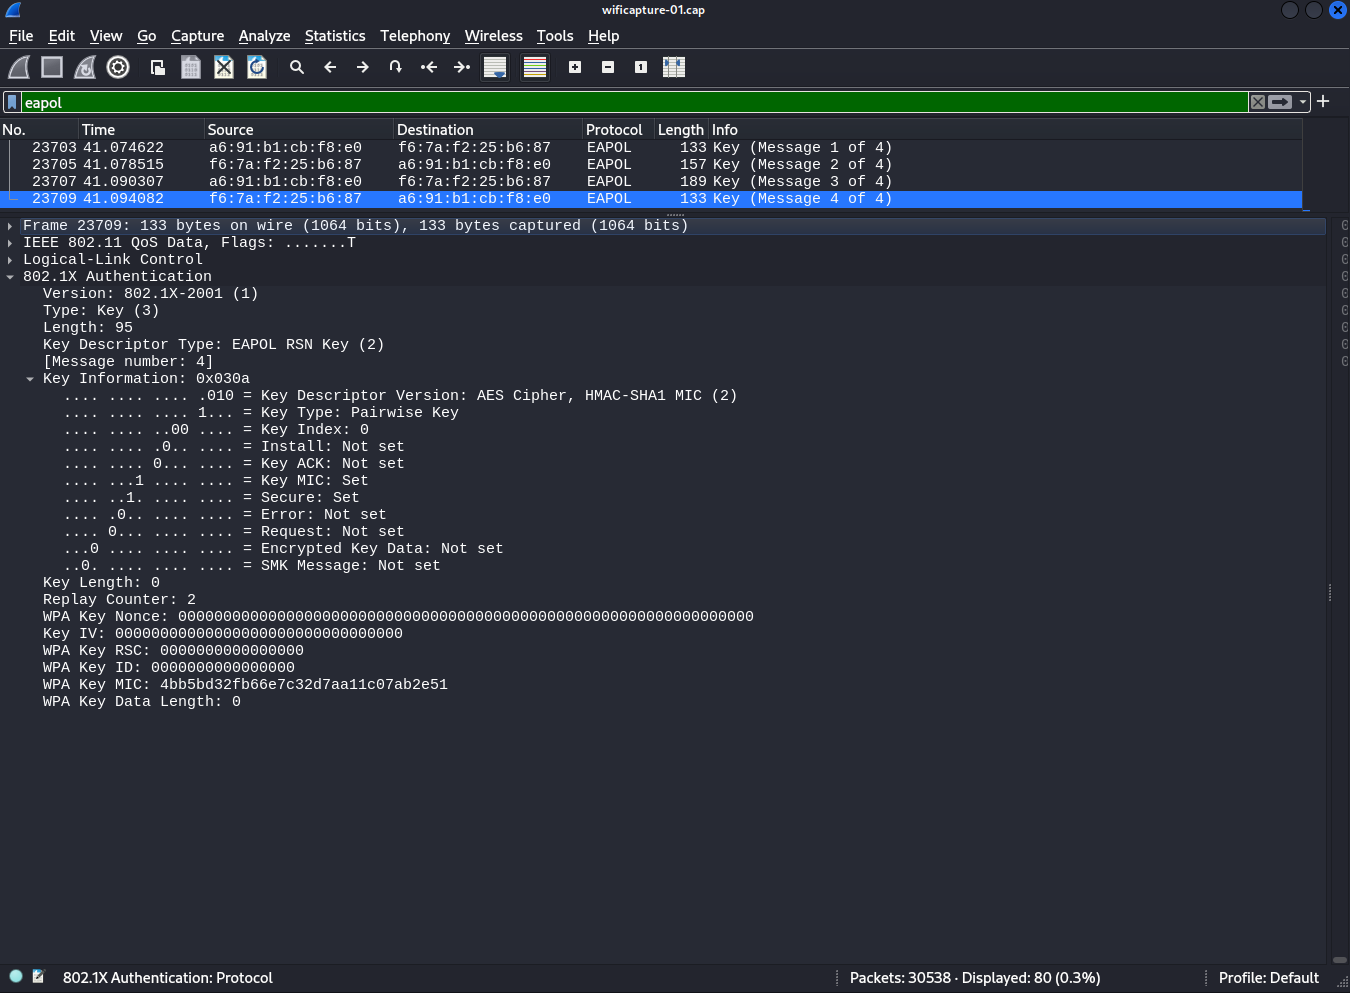
\includegraphics[width=0.8\linewidth]{images/msg4.png}
        \caption{Message 4: Client confirming the handshake completion.}
        \label{fig:msg4}
    \end{figure}
\end{enumerate}

By examining these messages in \texttt{Wireshark}, it was possible to confirm the integrity of the handshake. Each message plays a distinct role in ensuring a secure and authenticated connection, as described in the theoretical overview of the WPA2 Four-Way Handshake. The detailed inspection of the captured packets reinforced the understanding of the cryptographic mechanisms at play, providing valuable insights into the vulnerabilities associated with weak pre-shared keys.


    \item \textbf{Performing a Dictionary Attack:} Once the handshake was successfully captured, I proceeded with the dictionary attack to attempt to recover the password. Here’s the series of steps I followed:

    \begin{enumerate}
        \item \textbf{Extracting the RockYou Dictionary:} The first step was to extract the \texttt{rockyou.txt} dictionary file from its compressed archive. This was done using the command \textit{gunzip /usr/share/wordlists/rockyou.txt.gz}
        This command unzipped the compressed file, making the dictionary ready for use.

        \item \textbf{Initiating the Dictionary Attack:} With the handshake file and the dictionary prepared, I used the \texttt{aircrack-ng} tool to perform the attack. The command used was \textit{aircrack-ng wificapture.cap -w /usr/share/wordlists/rockyou.txt}
        
        Where:
        \begin{itemize}
            \item \texttt{-w}: Specifies the path to the wordlist (\texttt{rockyou.txt} in this case).
            \item \texttt{wificapture.cap}: The file containing the captured handshake.
        \end{itemize}

        \begin{figure}[h!]
            \centering
            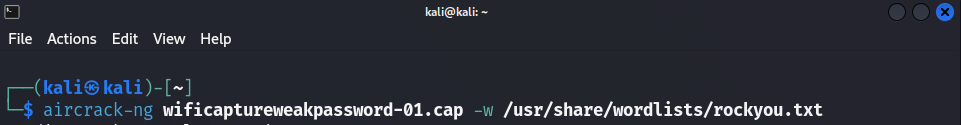
\includegraphics[width=0.8\linewidth]{images/rockyoucommand.png}
            \caption{Dictionary brute-force attack in progress.}
            \label{fig:rockyoucommand}
        \end{figure}

        \item \textbf{Waiting for the Process to Complete:} The \texttt{aircrack-ng} tool iteratively tested each password in the dictionary against the handshake data. Since the target network password was deliberately set to a simple passphrase for demonstration purposes, the tool successfully identified the password in a short amount of time. The output from \texttt{aircrack-ng} confirmed the recovered password, as shown in Figure \ref{fig:passwordfound}.

        \begin{figure}[h!]
            \centering
            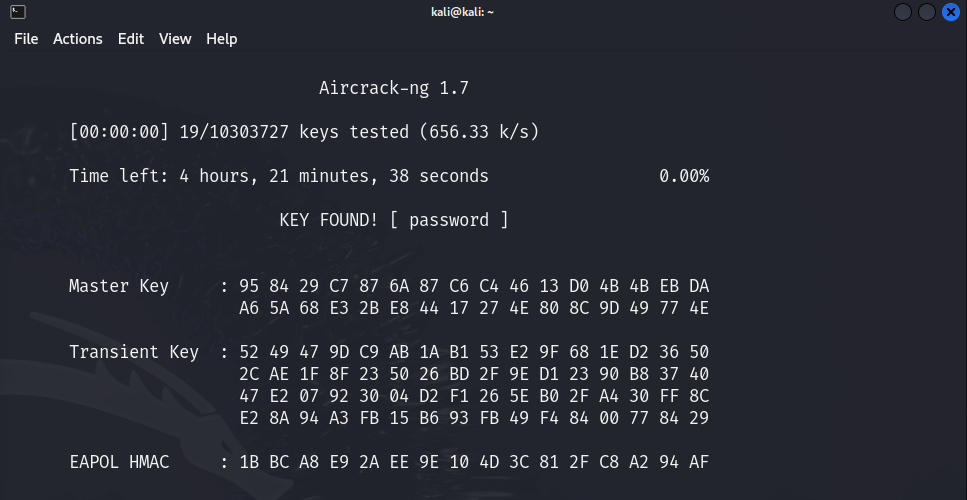
\includegraphics[width=0.8\linewidth]{images/passwordfound.png}
            \caption{Password successfully recovered using the dictionary attack.}
            \label{fig:passwordfound}
        \end{figure}
    \end{enumerate}
    
    This demonstration highlights the effectiveness of dictionary attacks against weak passwords and underscores the importance of using strong, unique passphrases to secure WPA2 networks.
    
\end{enumerate}


\section{Results and Analysis}
The deauthentication attack proved to be highly effective in demonstrating the vulnerabilities of WPA2 networks when weak passwords are employed. By sending deauthentication frames, the target client was successfully disconnected from the network. This action forced the client to attempt reconnection, triggering the WPA2 handshake. Using the `airodump-ng` tool, the handshake was captured with ease, confirming the effectiveness of this method in acquiring essential data for further analysis.

The next phase involved performing a dictionary attack on the captured handshake using `aircrack-ng`. The process relied on the `rockyou.txt` wordlist, a widely used dictionary for such purposes. Within a short period, the tool successfully recovered the network password. This success was largely due to the deliberately chosen weak password used in the demonstration, highlighting how easily poorly selected credentials can be compromised.

Overall, the experiment revealed that WPA2 networks with weak passwords are highly susceptible to such attacks. It underscores the importance of strong security measures to protect wireless communications from unauthorized access.

\section{Conclusion}
This study highlights the inherent vulnerabilities in WPA2 networks when secured with weak or easily guessable passwords. The deauthentication attack exploited the unauthenticated nature of deauthentication frames to disconnect a client, capturing the WPA2 handshake during its reconnection attempt. The subsequent dictionary attack demonstrated how attackers can leverage captured handshakes to recover passwords when weak credentials are used.

The results emphasize the necessity of adopting robust security practices, such as choosing strong, complex, and unique passwords to secure wireless networks. Additionally, the implementation of advanced security protocols like WPA3, which mitigates many of the weaknesses inherent in WPA2, is vital to ensuring the resilience of modern networks.

Through this practical demonstration, the chapter sheds light on the potential risks faced by wireless networks and the critical need for both users and administrators to prioritize security. A proactive approach to network configuration and encryption standards can significantly reduce the likelihood of such attacks succeeding.


\chapter{Evil Twin Attack Simulation}

This chapter presents the simulation of an Evil Twin attack, demonstrating the steps required to create a malicious network mimicking a legitimate access point (AP). The Evil Twin attack is commonly used to deceive users into connecting to a rogue network controlled by an attacker. This simulation focuses on setting up the Evil Twin network, with the limitation of having only one wireless network interface card (NIC). For a complete attack, two NICs are required: one to create the rogue AP and the other to perform DNS routing.

\section{Introduction to Evil Twin Attacks}
An Evil Twin attack involves creating a fake wireless AP with the same ESSID as the target network. This rogue network can be used to intercept user traffic, steal credentials, or inject malicious payloads. In this simulation, the focus is on creating the fake AP and executing a deauthentication attack to disconnect devices from the legitimate network, enticing them to connect to the Evil Twin.

\subsection{Tools and Software Utilized}
The following tools were utilized during the simulation:

\begin{itemize}
    \item \textbf{Airmon-ng}: To enable monitor mode on the wireless adapter.
    \item \textbf{Airodump-ng}: To scan for nearby networks and identify the target ESSID and channel.
    \item \textbf{Airbase-ng}: To create the Evil Twin network.
    \item \textbf{Aireplay-ng}: To execute the deauthentication attack.
\end{itemize}

\section{Objective and Methodology}
The objective of this simulation is to emulate an Evil Twin attack by creating a rogue network and demonstrating its visibility to nearby devices. The following steps outline the methodology:

\begin{enumerate}
    \item \textbf{Switching to Monitor Mode:} The first step involves enabling monitor mode on the wireless adapter. This allows the adapter to capture all wireless traffic in range. The command \texttt{sudo airmon-ng start wlan0} was used to switch the adapter from managed mode to monitor mode. Figure \ref{fig:monitor_mode} shows the output of this command.
    
    \begin{figure}[h!]
        \centering
        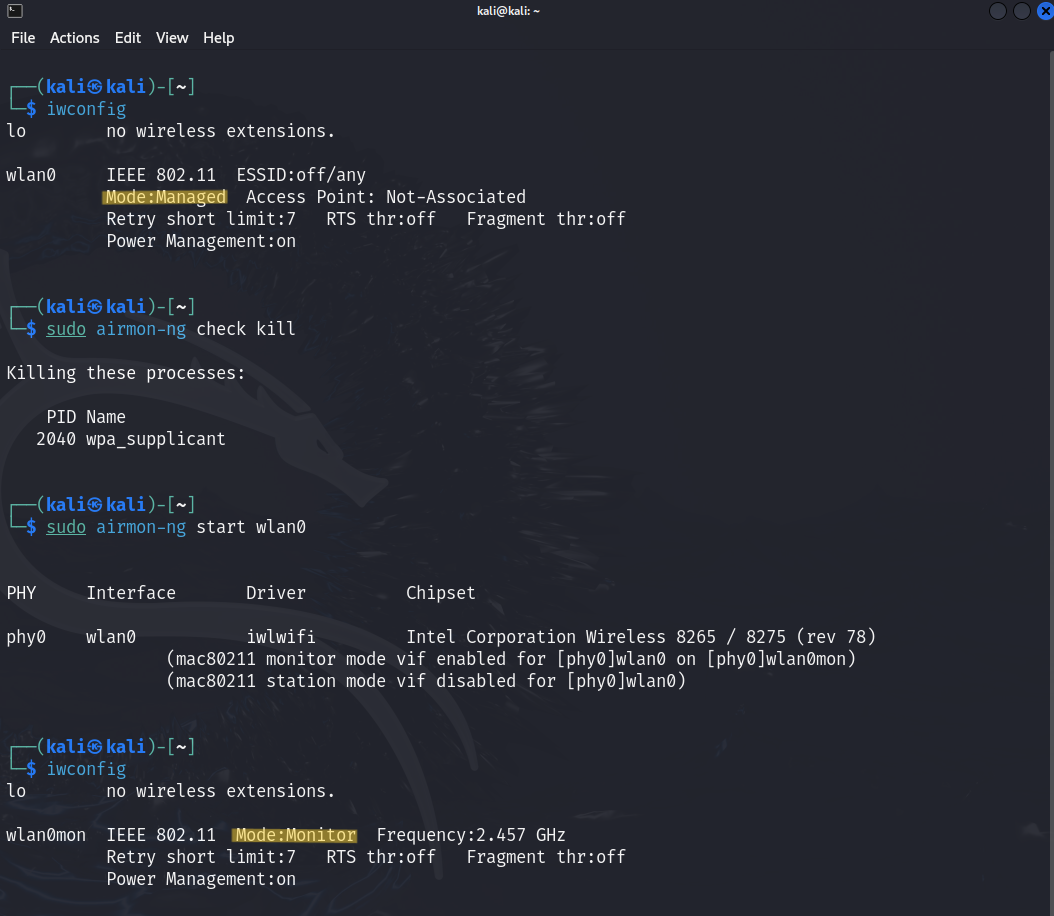
\includegraphics[width=0.8\linewidth]{images/wlanmon.png}
        \caption{Switching the network interface to monitor mode.}
        \label{fig:monitor_mode}
    \end{figure}

    \item \textbf{Scanning for Nearby Networks:} Using the \texttt{sudo airodump-ng wlan0mon} command, nearby wireless networks were scanned to identify the target network. The scan revealed the ESSID and channel of the target network, as shown in Figure \ref{fig:network_scan}.
    
    \begin{figure}[h!]
        \centering
        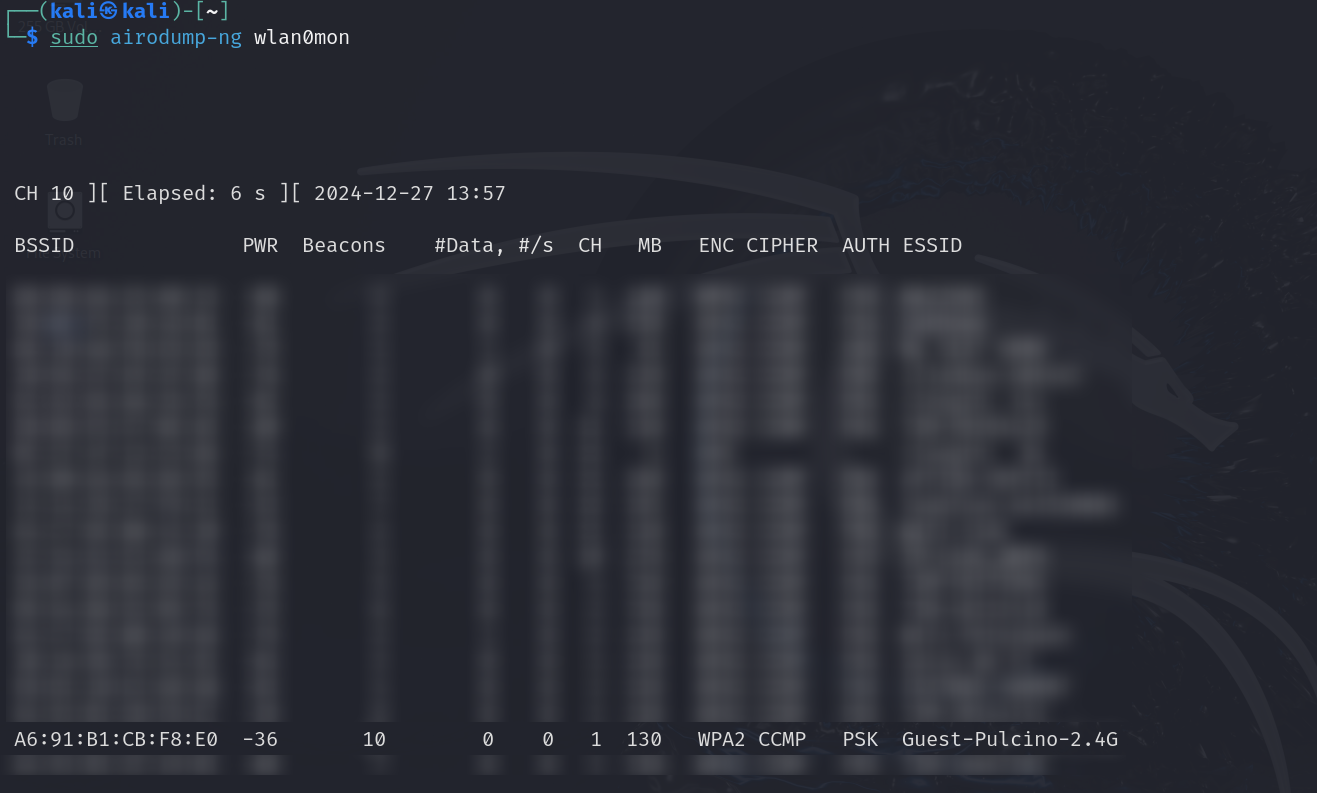
\includegraphics[width=0.8\linewidth]{images/networklist2.png}
        \caption{Scanning nearby networks to identify the target.}
        \label{fig:network_scan}
    \end{figure}

    \item \textbf{Creating the Evil Twin Network:} With the target network's ESSID and channel identified, the Evil Twin network was created using the following command: 
    \texttt{sudo airbase-ng -e TargetESSID -c Channel wlan0mon}. 
    The command output, displayed in Figure \ref{fig:evil_twin_creation}, confirms the successful creation of the rogue AP.
    
    \begin{figure}[h!]
        \centering
        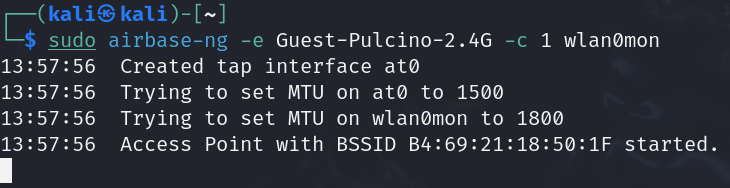
\includegraphics[width=0.8\linewidth]{images/evil_twin_creation.png}
        \caption{Creating the Evil Twin network with Airbase-ng.}
        \label{fig:evil_twin_creation}
    \end{figure}

    \item \textbf{Deauthentication Attack:} To disconnect clients from the legitimate network and prompt them to connect to the Evil Twin, a deauthentication attack was executed using the command:
    \texttt{sudo aireplay-ng --deauth 0 -a TargetBSSID wlan0mon}. 
    The process, as shown in Figure \ref{fig:deauth_attack}, involves sending deauthentication frames to all devices connected to the target network.
    
    \begin{figure}[h!]
        \centering
        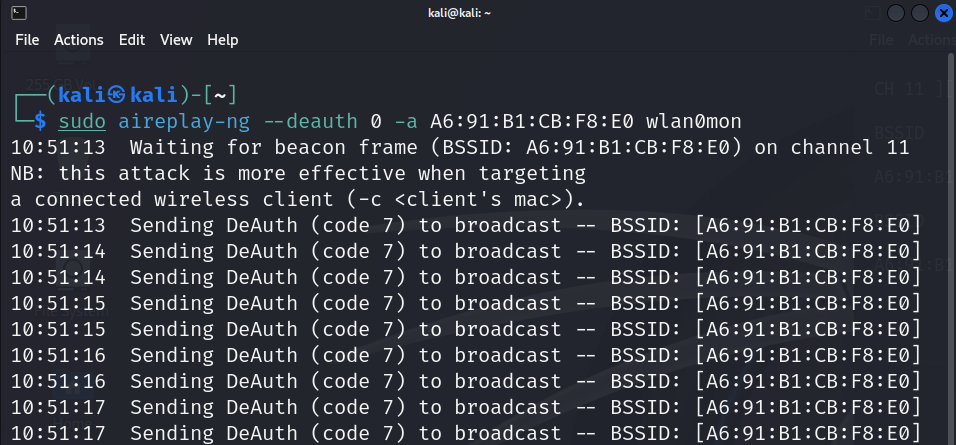
\includegraphics[width=0.8\linewidth]{images/dauth.png}
        \caption{Executing a deauthentication attack.}
        \label{fig:deauth_attack}
    \end{figure}

    \item \textbf{Testing Device Connection:} After the deauthentication attack, a mobile device was used to test the visibility of the Evil Twin network. Figure \ref{fig:device_connection} shows the mobile device successfully connecting to the rogue AP.
    
    \begin{figure}[h!]
        \centering
        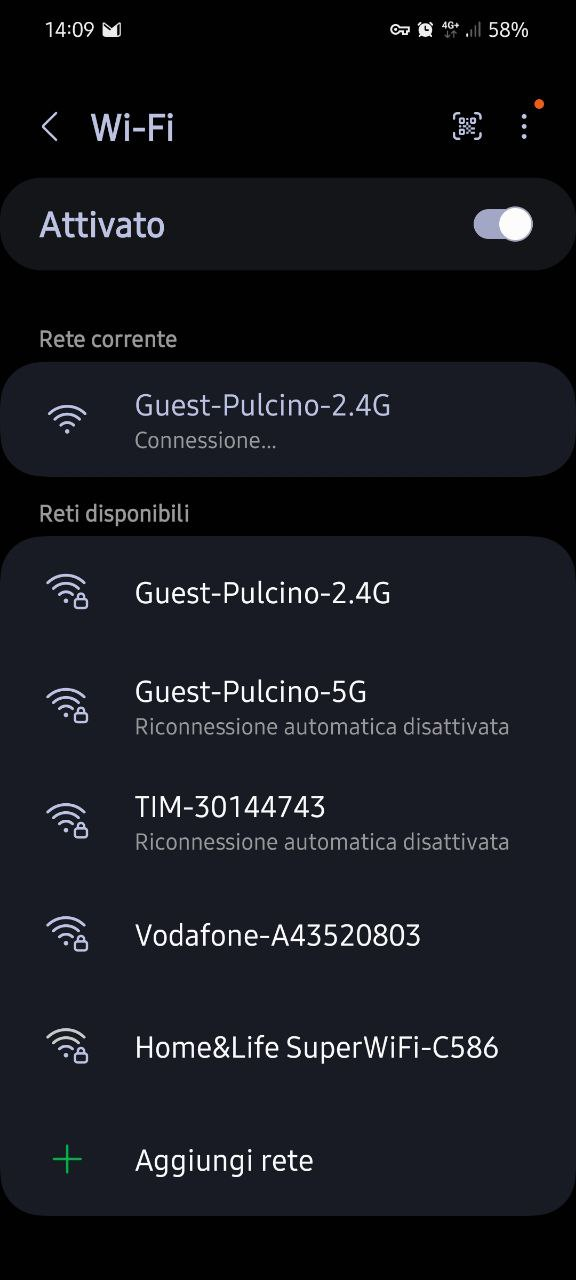
\includegraphics[width=0.5\linewidth]{images/device_connection.jpg}
        \caption{A mobile device connecting to the Evil Twin network.}
        \label{fig:device_connection}
    \end{figure}

    \item \textbf{Confirming the Connection:} The \texttt{airbase-ng} tool confirmed the successful connection of the device to the Evil Twin network, as depicted in Figure \ref{fig:connection_confirmation}.
    
    \begin{figure}[h!]
        \centering
        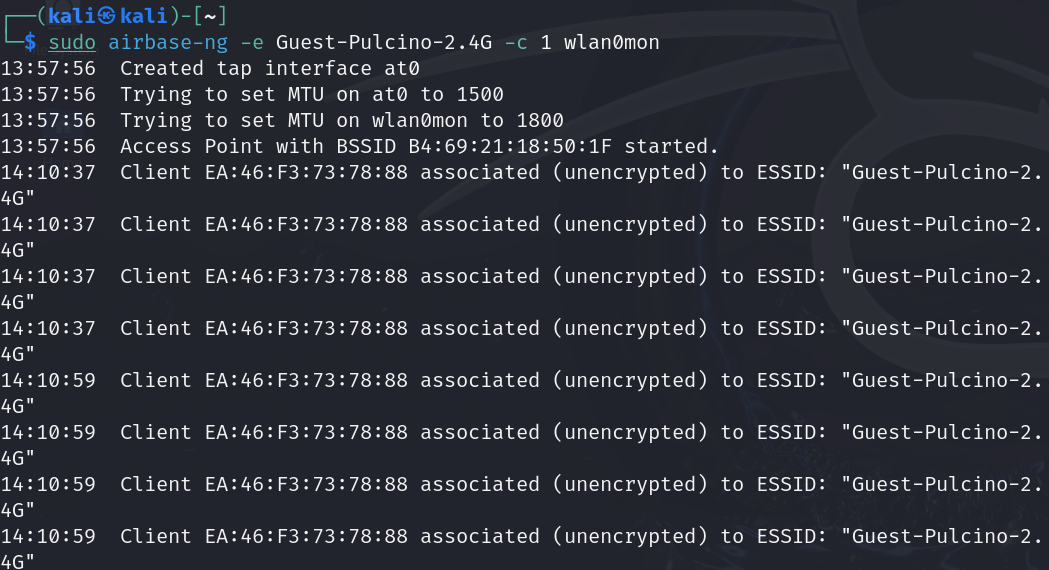
\includegraphics[width=0.8\linewidth]{images/connection_confirmation.png}
        \caption{Connection of the device confirmed by Airbase-ng.}
        \label{fig:connection_confirmation}
    \end{figure}

\end{enumerate}

\section{DNS Routing Configuration (Theoretical)}
To simulate a fully functional Evil Twin attack, DNS routing must be configured to redirect client requests. Although this step was not implemented in the current simulation due to the limitation of having only one NIC, the following commands are provided for completeness:

\begin{enumerate}
    \item Enable IP forwarding:\\
    \textit{echo 1 > /proc/sys/net/ipv4/ip_forward}

    \item Configure iptables for DNS redirection:\\
    \textit{iptables -t nat -A PREROUTING -p udp --dport 53 -j DNAT --to-destination 192.168.1.1}\\
    \textit{iptables -t nat -A POSTROUTING -j MASQUERADE}

    \item Start a DHCP server (e.g., \texttt{dnsmasq}) to assign IP addresses to connected devices.
\end{enumerate}

These commands illustrate the steps required to establish a functional rogue AP capable of routing and handling DNS requests.

\section{Results and Analysis}
The simulation successfully demonstrated the creation of an Evil Twin network and its visibility to nearby devices. The deauthentication attack effectively disconnected clients from the legitimate AP, encouraging them to connect to the rogue network. The results highlight the vulnerabilities of wireless networks to such attacks and the importance of implementing countermeasures, such as enabling WPA3 and monitoring for rogue APs.

\section{Conclusion}
This simulation emphasized the potential risks of Evil Twin attacks, even in a simplified setup. While the absence of DNS routing limited the scope of the attack, the exercise highlighted the ease with which an attacker can create a rogue AP to deceive users.

With the advent of WPA3, some vulnerabilities exploited in Evil Twin attacks have been mitigated. WPA3 introduces robust security features such as the Simultaneous Authentication of Equals (SAE) handshake, which replaces the WPA2 pre-shared key (PSK) authentication method. SAE is resistant to offline dictionary attacks and enhances the security of the authentication process. Additionally, WPA3 mandates the use of Protected Management Frames (PMF), which safeguard management frames like deauthentication and disassociation messages from being spoofed, thereby reducing the efficacy of deauthentication attacks.

However, it is important to note that the Evil Twin attack remains a critical issue regardless of the technology used on the access point. This is because the attack targets the user, not the network itself. Even with WPA3, a rogue AP can mimic a legitimate network’s ESSID and lure users into connecting to it. If a device is not configured to verify the server certificate (as in EAP-TLS or other enterprise-level configurations), users might still fall victim to such attacks. Furthermore, some legacy devices and networks that do not fully support WPA3 features may remain vulnerable.


\chapter{Analysis of Unencrypted Data Transmission on Open Networks}

In this section, we demonstrate the risks of transmitting sensitive information over unencrypted networks by simulating a scenario in which data is sent in plain text. This simulation aims to highlight the critical importance of encryption for securing communications in real-world applications.

\section{Setup and Methodology}

The experiment was conducted as follows:

\begin{enumerate}
    \item The encryption on the access point (AP) was disabled, rendering the network open and unprotected.
    \item Both an attacker device (the host computer) and a victim device were connected to this open network.
    \item On the attacker device, a simple HTTP website was hosted using Python with the following HTML code:
    
    \begin{adjustbox}{max width=\linewidth}
    \begin{lstlisting}[language=html]
    <!DOCTYPE html>
    <html lang="en">
    <head>
        <meta charset="UTF-8">
        <meta name="viewport" content="width=device-width, initial-scale=1.0">
        <title>HTTP Example</title>
    </head>
    <body>
        <h1>Welcome to an Unsecured HTTP Page</h1>
        <p>This is a demonstration of how data is sent in plain text over an unencrypted HTTP connection.</p>
        <form action="/submit" method="get">
            <label for="username">Username:</label>
            <input type="text" id="username" name="username">
            <br>
            <label for="password">Password:</label>
            <input type="password" id="password" name="password">
            <br>
            <button type="submit">Submit</button>
        </form>
    </body>
    </html>
    \end{lstlisting}
    \end{adjustbox}
    
    \item The victim device accessed the website through the open network and submitted credentials via the provided form.
    \item On the attacker device, Wireshark was used to capture and analyze the network traffic, revealing the transmitted username and password in plain text within an HTTP GET request.
\end{enumerate}

\section{Observed Results}

Using Wireshark, the attacker was able to intercept the network traffic and identify the HTTP GET request containing the user's credentials. Figure~\ref{fig:wireshark_capture} illustrates the intercepted request, showing the username and password in clear text. 

\begin{figure}[H]
    \centering
    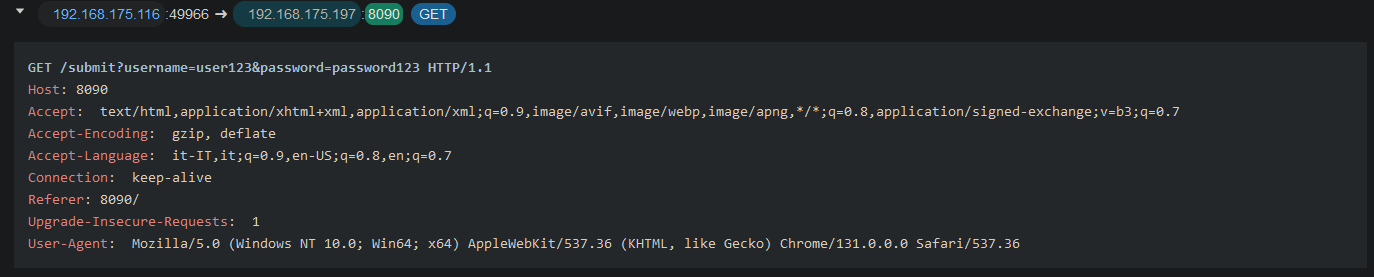
\includegraphics[width=\textwidth]{images/whiresharkcapture.png}
    \caption{Captured HTTP GET request showing transmitted credentials.}
    \label{fig:wireshark_capture}
\end{figure}

The lack of encryption allowed for the immediate identification of sensitive information, emphasizing the vulnerability of data transmission over open networks.

\subsection{Real-World Implications}

While this simulation was conducted in a controlled environment, it closely mimics real-world scenarios in which users connect to open networks, such as public Wi-Fi in cafes, airports, or other public spaces. In these environments, attackers can similarly exploit the absence of encryption to intercept sensitive information.

For example:
\begin{itemize}
    \item Users accessing websites without HTTPS encryption are vulnerable to attacks, such as credential theft or session hijacking.
    \item Even legitimate websites may inadvertently expose users if their login forms rely on HTTP instead of HTTPS.
\end{itemize}

This simulation underscores the vital importance of encryption protocols, such as HTTPS, in securing data transmission. By encrypting the content, these protocols ensure that sensitive information cannot be easily intercepted or interpreted, highlighting the indispensable role of cryptography in modern network security.


\section{Conclusion}

The experiment demonstrates how unencrypted networks pose significant risks to user data. It serves as a strong argument for adopting encryption protocols, such as WPA3 for wireless networks and HTTPS for web communication, to protect sensitive information.

Encryption is no longer optional but a fundamental requirement for ensuring data security in today's interconnected world.

\chapter{Conclusion}

This project has explored the vulnerabilities and security challenges associated with wireless networks, focusing on the WPA2 protocol. Through three interconnected simulations, both theoretical and practical aspects of wireless security were analyzed, shedding light on the risks posed by insufficient protection and outdated configurations.

The first simulation demonstrated the vulnerability of the WPA2 four-way handshake to brute-force attacks, emphasizing the critical need for strong and complex passwords. By capturing the handshake and successfully executing a dictionary attack, the experiment highlighted how attackers can exploit weak credentials, even in networks utilizing advanced encryption standards like AES.

The second simulation illustrated the creation of an Evil Twin access point, a common attack vector used to deceive users into connecting to a rogue network. This experiment showcased the risks posed by user behavior and the lack of server certificate verification in some configurations. Although the simulation was limited by hardware constraints, it effectively demonstrated the feasibility of such an attack, further reinforcing the importance of user education and advanced authentication protocols.

The final simulation focused on unencrypted networks, showing how sensitive data, such as usernames and passwords, can be intercepted when transmitted over open Wi-Fi. By analyzing HTTP traffic with Wireshark, the experiment underscored the importance of encryption protocols like HTTPS and the necessity of securing public and private networks to protect user data from potential eavesdroppers.

These experiments collectively highlight several key takeaways:
\begin{itemize}
    \item The importance of adopting strong passwords and modern security protocols, such as WPA3, to mitigate vulnerabilities.
    \item The need for user awareness about the risks of connecting to open or suspicious networks and the dangers of transmitting sensitive information without encryption.
    \item The critical role of encryption protocols, such as HTTPS and TLS, in securing online communications.
\end{itemize}

While the simulations were conducted in a controlled environment, they mimic real-world scenarios where attackers exploit common weaknesses in wireless networks. The findings underscore the necessity for continuous advancements in wireless security standards, as well as proactive measures by both network administrators and end users.

Future work could explore the implementation of WPA3, which introduces significant improvements in authentication and encryption mechanisms. Additionally, more advanced simulations could include the integration of intrusion detection systems and the analysis of enterprise-level security measures, such as EAP-TLS.

By combining theoretical knowledge with practical experimentation, this project provides a comprehensive understanding of wireless security vulnerabilities and offers insights into best practices for safeguarding modern networks. Wireless security remains a dynamic field, and as technology evolves, so must our approach to protecting sensitive information in an increasingly connected world.


% ----------------------
% ---- BIBLIOGRAPHY ----
% ----------------------
\backmatter
\printbibliography[heading=bibintoc, title=Bibliografia/Sitografia]
\sloppy % serve a non far andare i link oltre ai margini
% ----------------------
% ---- DOCUMENT END ----
% ----------------------
\end{document} % Fine documento
